\chapter{Microservice-Infrastruktur}
\label{chap:microserviceinfrastruktur}

\section{Monorepo und Submodules}
\label{sec:monorepoundsubmodules}
% Git submodules

\section{Infrastruktur}
\label{sec:infrastruktur}

\begin{figure}
    \label{figure:microserviceinfrastruktur}
    \begin{center}
    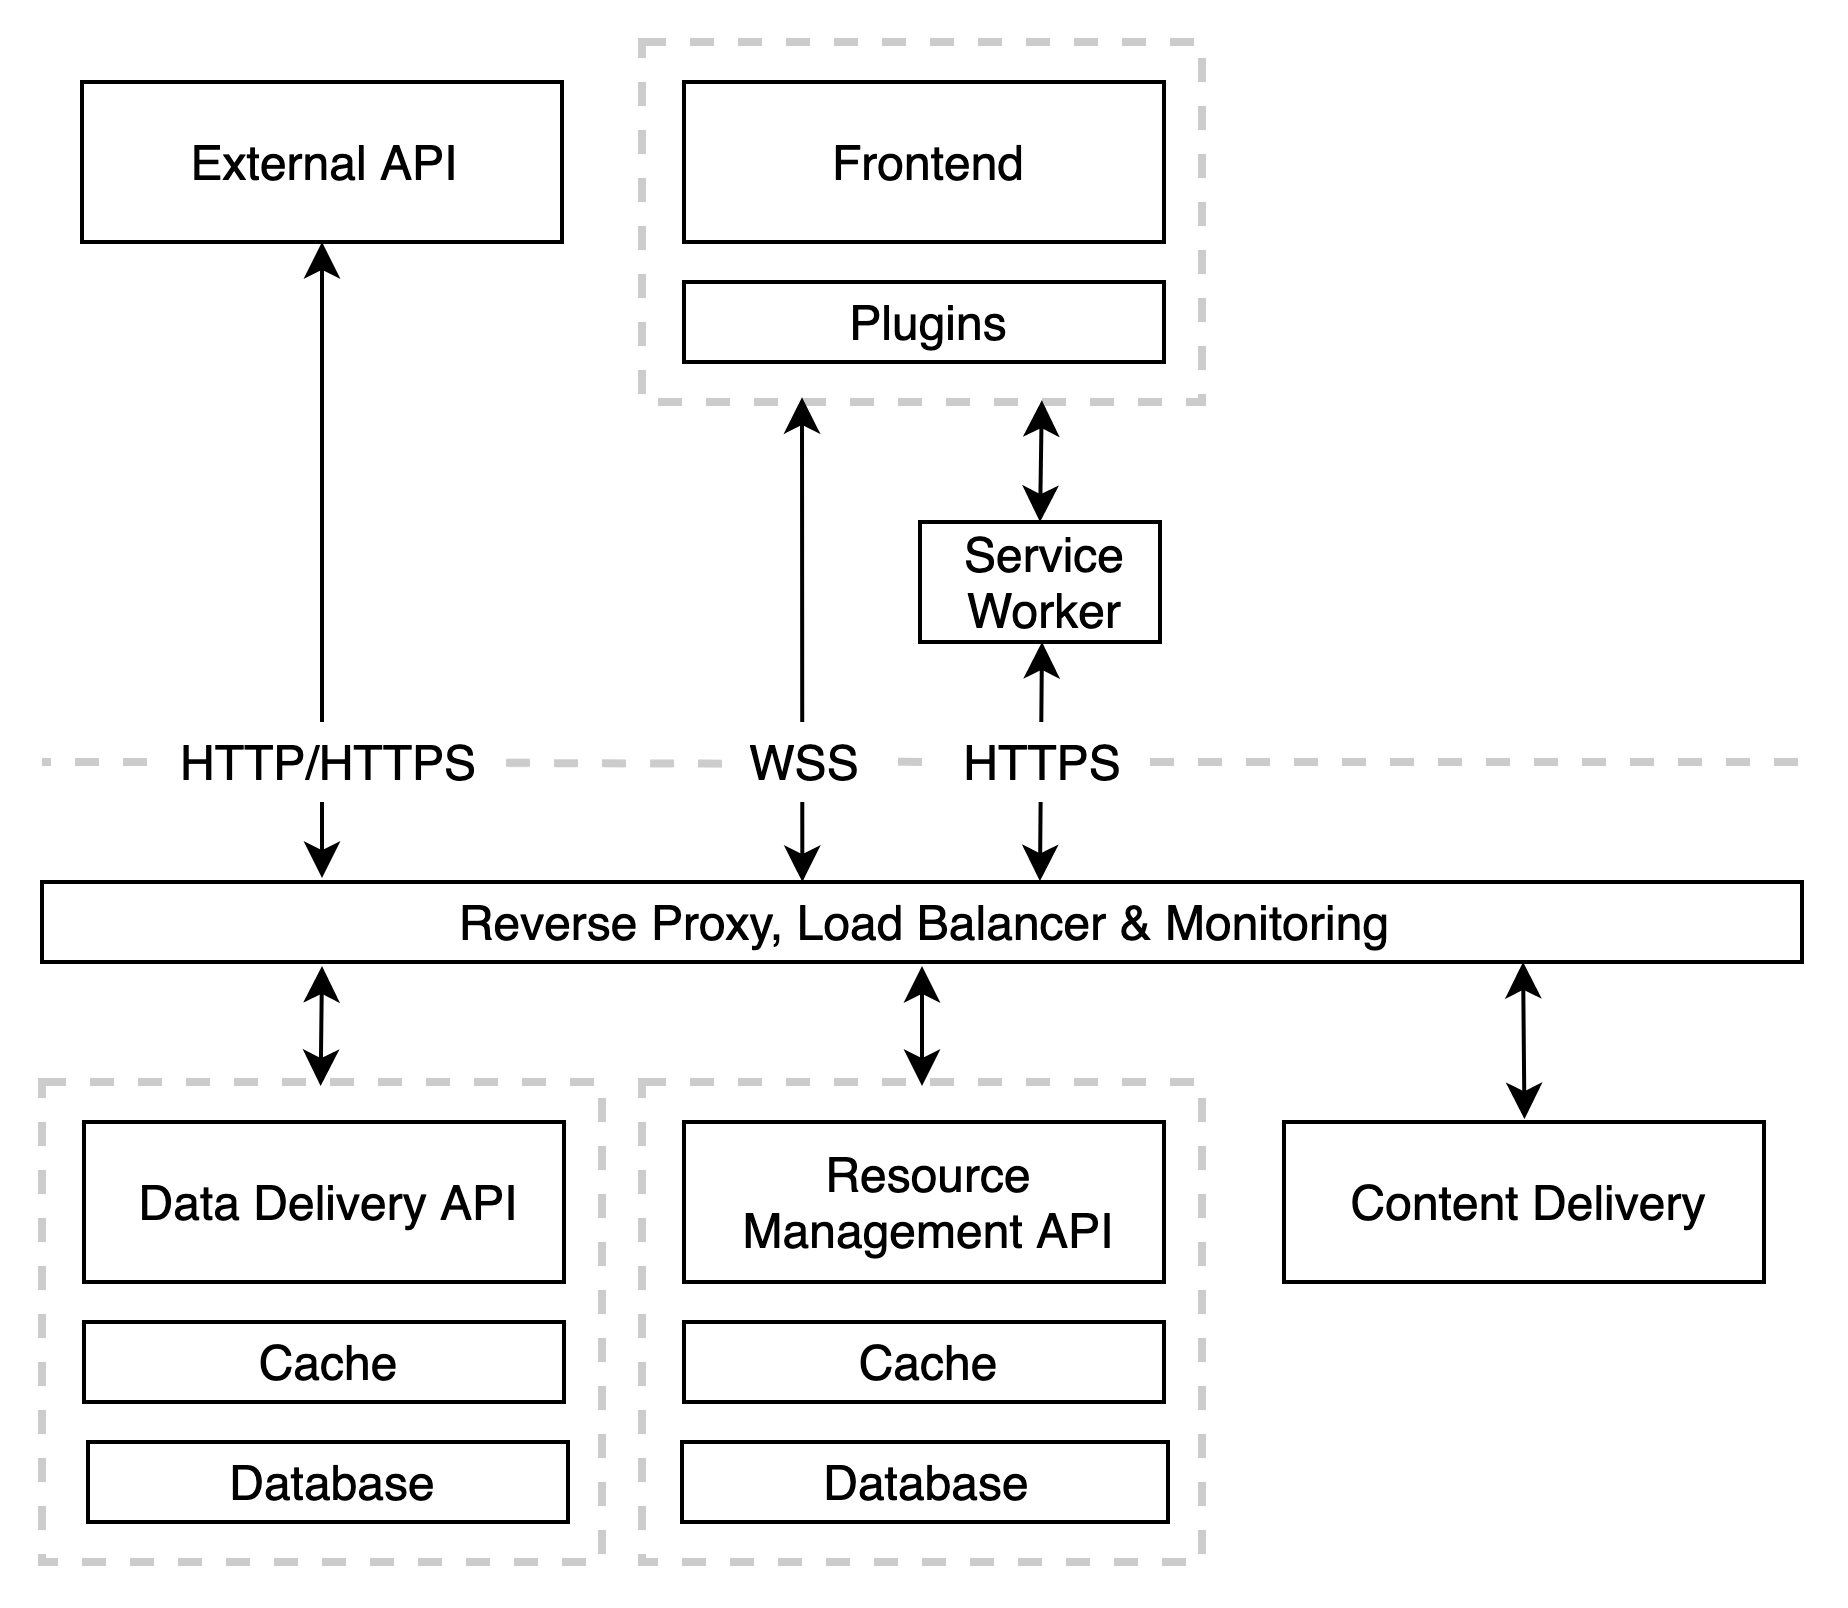
\includegraphics[scale=0.2]{img/abbildungen/MicroserviceInfrastruktur}
    \end{center}
    \caption{Übersicht über die Microservice-Infrastruktur}
\end{figure}

\subsection{Gitlab CE}
\label{subsec:gitlabce}
% Die Unabhängigkeit gegenüber einzelner Unternehmen
\subsection{Gitlab Runner}
\label{subsec:gitlabrunner}

\subsection{Docker Registry}
\label{subsec:dockerregistry}

\subsection{Hetzner Cloud}
\label{subsec:hetznercloud}

\section{Pipeline Design}
\label{sec:pipelinedesign}

\subsection{Umgebungsvariablen}
\label{subsec:umgebungsvariablen}

\subsection{Stages}
\label{subsec:stages}
% Continuous Integration mit Gitlab

\subsection{Docker Compose Setup}
\label{subsec:dockercomposesetup}

\subsection{Health-Checks}
\label{subsec:healthcheck}
In Microservice-Infrastrukturen sind die einzelnen Services eng miteinander verknüpft
und voneinander abhängig. Um die Verfügbarkeit sicherzustellen, werden auf
Serviceebene Healthcheckendpunkte bereitgestellt. Diese spiegeln den aktuellen
Gesundheitszustand des jeweiligen Dienstes wieder. Ein Healthcheckendpunkt
ist speziell dann nützlich, wenn ein Dienst oder ein Verfahren von einem anderen
abhängig ist. So ist beispielsweise die Backendapi von der Datenbank
abhängig. Andererseits ist der Frontenddienst sowie das Apitestverfahren
in der Buildpipeline von der Backendapi abhängig. 

\begin{listing}
    \label{lst:healthcheck}
    \inputminted{sh}{snippets/sh/healthcheck.sh}
    \caption{Healthcheckbeispiel in der Gitlab CI}
\end{listing}

\section{Reverse Proxy}
\label{sec:reverseproxy}

\section{Load Balancer}
\label{sec:loadbalancer}

\section{Inhaltsauslieferung}
\label{sec:inhaltsauslieferung}

\subsection{Kompression}
\label{subsec:kompression}

\subsection{CDN}
\label{subsec:cdn}

\section{Monitoring}
\label{sec:monitoring}

\section{Wartung}
\label{sec:wartung}
% clean up von server und docker setup

\subsection{Skizzen der Infrastruktur}
\label{subsec:skizzenderinfrastruktur}

% Wahl der Technologien, Tech-Stack?
% Anforderungen an die Technologien
% Umfeld etc
% Geschwindigkeit der Entwicklung
